
% !TeX root=DeepRelAttr.tex
% !TEX TS-program = pdfLatex

%%%%%%%%%%%%%%%%%%%%%%% END-TO-END DEEP RELATIVE ATTRIBUTES %%%%%%%%%%%%%%%
\section{Proposed Method}
\label{sec.3}

We propose to use a ConvNet based deep neural network that is trained to optimize the appropriate ranking loss for the task of predicting relative attribute strength. The network architecture consists of two parts, the \textit{feature learning and extraction} part and the \textit{ranking} part.

The feature learning and extraction part takes an image, $I_i$, as input and outputs the learned feature representation for that image $\psi_i \in \mathcal{R}^d$.
% (Figure \ref{fig.2}).
Different methods have been developed in the literature, for extracting and leaning features in a deep framework. The outputs of some intermediate layer of a state-of-the-art ConvNet architecture, such as AlexNet \cite{krizhevski}, VGGNet \cite{verydeep} or GoogleNet \cite{googlenet},
% can be counted as learned features.
can be used.
% Here, we have incorporated VGGNet and its fc7 layer, and learned the attribute-specific features. 

% In our experiments we use the fc7 (the last layer before the probability layer) of VGG-16 \cite{verydeep} as the feature extraction part of the network.

For the ranking part, we can use any ranking procedure that accepts relatively ordered pairs of feature vectors as input, and maps each feature vector to an absolute ranking. The main objective would be to obtain a model, trained by a set of relatively compared pairs of images for any specific attribute. This model will then be used to determine the absolute ranking of a novel unseen test image among all the trained images. One of the most widely used strategies in the literature is RankSVM \cite{Joachims2002}. However, here, we propose a ranking strategy with a similar structure as in the feature learning part, so that we can fine-tune the parameters of the feature learning part, while learning the ranking function. To this end, our proposed ranking part enjoys a neural network architecture. Burges \etal~\cite{Burges2005} introduced a ranking procedure using gradient descent. We use a similar procedure (known as RankNet), in which the learned features are fed into, and then a back-propagation strategy fine-tunes the parameters of the feature learning part. Intertwining these two procedures helps learning fine-tuned and attribute-specific features, while ranking the images with respect to the attributes. 
%It can be learned through gradient descent, thus  that with pairs of features vectors with relative ordering or similar strength of a particular attribute, learns to map each feature vector to an absolute ranking of that feature vector, that can be used to predict the relative ordering of each pairs of test feature vectors. Further more we need the ranking part to be learnable by gradient descent, so that using back-propagation we can learn (or fine-tune) the parameters of the feature extraction part of the network.
% One such architecture RankNet \cite{Burges2005} which is used in our proposed method is presented in detail below.
%For the ranking part we propose to use RankNet, the award winning work of Burges \etal \cite{Burges2005}, which is described in detail below.

% The ranking part, maps the feature representation $\psi_i$ to the attribute strength or absolute rank of the input $r_i \in \mathcal{R}$. Then given two attribute strengths generates the posterior $P_{ij}$ that the strength of the attribute in $I_i$ is larger than the strength of the attribute in $I_j$. 

In the following, the two parts of the proposed framework are explained in details.

\subsection{RankNet: Learning to Rank Using Gradient Descent}\label{sec3.1}
Given a set of pairs of sample feature vectors $\big\{( \psi_{1}^{(k)}, \psi_{2}^{(k)} ) | k \in \{1, ...,n\} \big\} \in \mathbb{R}^{d \times d}$ and target probabilities $\big\{ t_{12}^{(k)} | k \in \{1, ...,n\} \big\}$, that sample $\psi_{1}^{(k)}$ is to be ranked higher than sample $\psi_{2}^{(k)}$, we want to learn a ranking function $f : \mathbb{R}^d \mapsto \mathbb{R}$, such that %the values of
$f$ specifies the ranking order of a set of features. Here, $f(\psi_i) > f(\psi_j)$ indicates that the model has learned feature vector $\psi_i$ with higher rank than $\psi_j$, denoted by $\psi_i \triangleright \psi_j$. The RankNet model \cite{Burges2005} provides an elegant way to deal with this.

Denoting $r_i \equiv f(\psi_i)$, RankNet models the mapping from rank estimates to posterior probabilities $P_{ij} = P(\psi_i \triangleright \psi_j)$ using a logistic function 
$$
P_{ij} \equiv \frac{1}{1 + e^{-(r_i - r_j)}}.
$$

The loss for the sample pair of feature vectors $(\psi_i, \psi_j)$ along with target probability $t_{ij}$ is defined as
$$
C_{ij} \equiv - t_{ij} \log (P_{ij}) - (1 - t_{ij}) \log (1 - P_{ij}),
$$
which is the binary cross entropy loss.
Figure \ref{fig.2} plots the loss value $C_{ij}$ as a function of $r_i - r_j$ for three values of target probability $t_{ij} = \{0, 0.5, 1\}$.

\begin{figure}
\centering
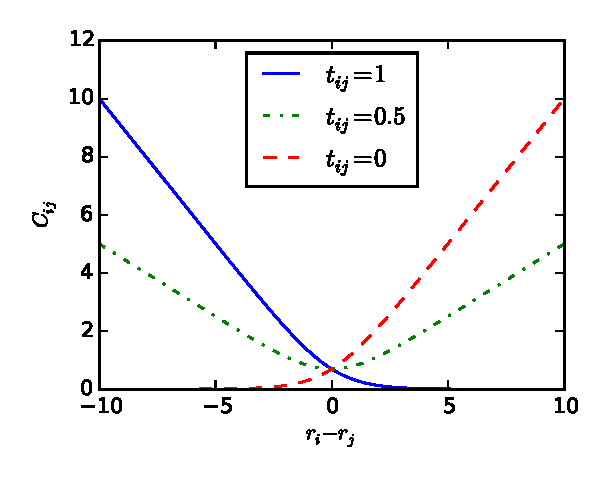
\includegraphics[width=8cm]{fig2-2/fig3.eps}
\caption{The loss value for three values of the target probability.}
\label{fig.2}
\end{figure}

Note that when $t_{ij} = 0.5$, and no information is available about the relative rank of the two samples, the cost becomes symmetric. This can be used as a way to train on patterns that are desired to have similar rank. This is somewhat scarce in the previous works on relative attributes, where the relation between the attributes were mostly considered to be less or greater. In other words, in the previous works, equality relation was not much explored.
This model asymptotes to a linear function which makes it more appropriate for problems with noise labels than quadratic loss functions.

Training this model is done using stochastic gradient descent.%, which is also used in our proposed method.
For testing, we only need to estimate the value of $f(\psi_i)$, which resembles the absolute rank of the test sample.

\subsection{Deep Relative Attributes}\label{sec3.2}

%%%%%%%%%%%%%%%%%%%%%%%% Figure 2 %%%%%%%%%%%%%%%%%%%%%%%%%%%%%%%%%%%%%%%%%%%%%%%%%%%%%
\begin{figure*}
\centering
\scalebox{.3}
{
% We need layers to draw the block diagram
\pgfdeclarelayer{background}
\pgfdeclarelayer{foreground}
\pgfsetlayers{background,main,foreground}

% Define a few styles and constants
\tikzstyle{sensor}=[draw, fill=blue!20, text width=5em, 
    text centered, minimum height=2.5em]
\tikzstyle{ann} = [above, text width=5em]
\tikzstyle{naveqs} = [sensor, text width=6em, fill=red!20, 
    minimum height=12em, rounded corners]
\def\blockdist{2.3}
\def\edgedist{2.5}

\begin{tikzpicture}
    % feature extraction part rectangle
	\node [scale=3] (testtitle) at (10.5cm, 5.0cm) {\textcolor{red}{Test time}};
	\draw [rounded corners=1cm, dashed, line width=3, red] (-3.5cm, 4cm) rectangle (24.5cm,-2.5cm);
	% images
	\node (im1) at (0cm,1cm) [draw] {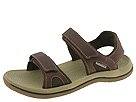
\includegraphics[scale=1]{Fig2/im1.jpg}};
	\node (im2) at (0cm, -6cm) [draw] {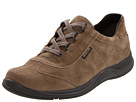
\includegraphics[scale=1]{Fig2/im2.jpg}};

	% topconv1 layer
	\node (tconv1) at (5.1cm, 1cm) {};
%	\draw [fill=blue!20] (5.6cm,3.1cm) rectangle (9.6cm,0.1cm);
	\draw [fill=blue!20] (5.4cm,2.9cm) rectangle (9.4cm,-0.1cm);
	\draw [fill=blue!20] (5.2cm,2.7cm) rectangle (9.2cm,-0.3cm);
	\draw [fill=blue!20] (5cm,2.5cm) rectangle (9cm,-0.5cm);

	% bottomconv1 layer
	\node (bconv1) at (5.1cm, -6cm) {};
%	\draw [fill=blue!20] (5.6cm,-3.9cm) rectangle (9.6cm,-6.9cm);
	\draw [fill=blue!20] (5.4cm,-4.1cm) rectangle (9.4cm,-7.1cm);
	\draw [fill=blue!20] (5.2cm,-4.3cm) rectangle (9.2cm,-7.3cm);
	\draw [fill=blue!20] (5cm,-4.5cm) rectangle (9cm,-7.5cm);

	% arrows from images to conv1s
	\path [draw, ->, line width=3] (im1.east) -- node [above, scale=3] {$I_i$} (tconv1);
	\path [draw, ->, line width=3] (im2.east) -- node [above, scale=3] {$I_j$} (bconv1);

	% topconv2 layer
	\node (tconv2) at (12cm, 1cm) {};
	\draw [fill=blue!20] (12.6cm,3.1cm) rectangle (16.6cm,0.1cm);
	\draw [fill=blue!20] (12.4cm,2.9cm) rectangle (16.4cm,-0.1cm);
	\draw [fill=blue!20] (12.2cm,2.7cm) rectangle (16.2cm,-0.3cm);
	\draw [fill=blue!20] (12cm,2.5cm) rectangle (16cm,-0.5cm);

	% bottomconv2 layer
	\node (bconv2) at (12cm, -6cm) {};
	\draw [fill=blue!20] (12.6cm,-3.9cm) rectangle (16.6cm,-6.9cm);
	\draw [fill=blue!20] (12.4cm,-4.1cm) rectangle (16.4cm,-7.1cm);
	\draw [fill=blue!20] (12.2cm,-4.3cm) rectangle (16.2cm,-7.3cm);
	\draw [fill=blue!20] (12cm,-4.5cm) rectangle (16cm,-7.5cm);

	\path (tconv1.east)+(4.65cm, 0cm) -- node [scale=4]{\dots} (tconv2);
	\path (bconv1.east)+(4.65cm, 0cm) --node [scale=4]{\dots} (bconv2);

	\node (convnet) [below, scale=3.5] at (11cm, -8cm) {ConvNet};

	% toprank
	\node (tconvout) at (16.6cm, 1cm) {};
	\node (trank) at (20.5cm, 1cm) [rectangle, draw, fill=red!20, scale=3, align=center] {Ranking \\  Layer};
	\path [draw, line width=3, ->] (tconvout) -- node[above, scale=3] {$\psi_i$} (trank.west);

	% bottomrank
	\node (bconvout) at (16.6cm, -6cm) {};
	\node (brank) at (20.5cm, -6cm) [rectangle, draw, fill=red!20, scale=3, align=center] {Ranking \\  Layer};
	\path [draw, line width=3, ->] (bconvout) -- node[above, scale=3] {$\psi_j$} (brank.west);

	% shared rank layer
	\node (dashcenter) at (10.75cm, 0cm) {};
	\path [draw, line width=2, <->] (trank.south) -- node [scale=2, draw, rectangle, fill=white, line width=0] {\rotatebox{90}{shared}} (brank.north);
	\path [draw, line width=2, <->] (trank.south -| dashcenter) -- node [scale=2, draw, rectangle, fill=white, line width=0] {\rotatebox{90}{shared}} (brank.north -| dashcenter);

	% posterior
	\node (posterior) at (26cm, -2.5cm) [rectangle, draw, fill=orange!10, scale=3, minimum width=15] {\rotatebox{90}{Posterior}};

	% connect rank layer to posterior
	\path [draw, line width=2, ->] (trank.east) -- node [scale=3, above] {$r_i$} (posterior);
	\path [draw, line width=2, ->] (brank.east) -- node [scale=3, above] {$r_j$} (posterior);

	% BXE
	\node (bxent) at (36cm, -2.5cm) [draw,fill=green!10, regular polygon, regular polygon sides=3, shape border rotate=-90, scale=8, line width=2] {};
	\node at (36.2cm, -2.5cm) {\Huge BXEnt};

	% target value
	\node (target) at (29cm , -4.2cm) [scale=3] {target};

	% connect to bxe
	\draw [line width=3, ->] (posterior.east) -- ++(2cm, 0cm) |- node [above right, scale=3] {$p_{ij}$}  (bxent.north west);
	\draw [line width=3, ->] (target.east) -- node [below, scale=3] {$t_{ij}$}  (bxent.south west |- target.east);

	% loss node
	\node (loss) [scale=3] at (45cm, -2.5cm) { loss};

	% connect bxent to loss
	\draw [line width=3, ->] (bxent.east) -- node [above, scale=3] {$C_{ij}$}  (loss.west);
\end{tikzpicture}}
\caption{The overall schematic view of the proposed method during training. During test time a sub-network annotated with the red dotted box is used. The network consists of two parts, the \textit{feature extraction} part (labeled ConvNet in the figure), and the \textit{ranking} part.}
\label{fig.3}
\end{figure*}
%%%%%%%%%%%%%%%%%%%%%%%% Figure 2 %%%%%%%%%%%%%%%%%%%%%%%%%%%%%%%%%%%%%%%%%%%%%%%%%%%%%

Our final model is depict in figure \ref{fig.3} which is trained for each attribute separately. During training pairs of images $(I_i, I_j)$ are presented to the network, together with the target probability $t_{ij}$. If $I_i \triangleright I_j$ for the attribute, then $t_{ij}$ is  set to be larger than $0.5$ depending on our confidence on the relative ordering of $I_i$ and $I_j$. Similarly if $I_i \triangleleft I_j$, then $t_{ij}$ is set to be smaller than $0.5$ and if it is desired that the two images have the same rank, $t_{ij}$ is set to $0.5$. Because of the nature of the datasets we chose $t_{ij}$ from the $\{1, 0.5, 0 \}$ set according to the annotations of the dataset.

The pair of images then go though the feature learning and extraction part of the network (ConvNet) that maps the images into feature vectors $\psi_i$ and $\psi_j$. Further these feature vectors go through the ranking layer as described in section \ref{sec3.1}. We choose the ranking layer to be a fully connected neural network layer with linear activation function, 1 output neuron and parameters $w$ and $b$ that maps the feature vector $\psi_i$ to the estimated absolute rank of that feature vector $r_i$ where
$$
r_i \equiv w^T x + b
$$
and $r_i \in \mathbb{R}$.
The two estimate ranks are then combined to output the estimated posterior probability $P(\psi_i \triangleright \psi_j)$ and is used along with the target probability $t_{ij}$ to calculate the loss. This loss is then back-propagated through the network and is used to update the parameters of the whole network including both the parameters of the feature learning and extraction sub-network and the ranking layer.

During test time, as shown in Figure \ref{fig.3}, we only need to calculate the estimated absolute rank $r_i$ for each test image $I_i$. Using these estimated absolute ranks we can then easily predict the relative attribute strength for all test pairs.